\documentclass{article}
\usepackage[utf8]{inputenc}
\usepackage[spanish]{babel}
\usepackage{listings}
\usepackage{graphicx}
\graphicspath{ {images/}}
\usepackage{cite}

\begin{document}

\begin{titlepage}
    \begin{center}
        \vspace*{1cm}
            
        \Huge
        \textbf{Parcial I Informtica II Informe}
            
        \vspace{0.5cm}
        \LARGE
            
        \vspace{1.5cm}
            
        \textbf{Integrantes:}
        \\
        \vspace{1.5cm}
        \textbf{Daniel Andres Agudelo Garcia}
        \\
        \textbf{Andres Felipe Rendon Villada} \\
        \textbf{Esteban Felipe Guiza Piñeros}
        
            
        \vfill
            
        \vspace{0.8cm}
            
        \Large
        Despartamento de Ingeniería Electrónica y Telecomunicaciones\\
        Universidad de Antioquia\\
        Medellín\\
        Marzo de 2021
            
    \end{center}
\end{titlepage}

\tableofcontents

\vspace{13cm}

\section{Introduccion: Analisis del problema}

Leimos el informe del problema y las soluciones que se necesitaban, se hizo un analisis con todos las posibles soluciones que sean factibles para seguir el paso a paso estipilado del informe.

 \vspace{1cm}
 
 
Obervamos la problematica a tener en cuenta, en la cual planteamos diferentes soluciones y elegimos la mas optima, pensando en un desarrollo ideal a la propuesta hecha, formando una idea de proyecto y estructurando las mecanicas y/o codigos a implementar, tomando como eje principal que el usuario pueda ingresar el numero que desee de patrones a generar y cualquier patron.
 \vspace{1cm}

Al tener las soluciones planteadas, buscamos e investigamos todos los conceptos que vamos a necesitar para el montaje del circuito en tinkercar, al igual que entender el funcionamiento de todos sus componentes para tener conciencia de como lo vamos a utilizar.






\vspace{14cm}

\section{Desarrollo} \label{contenido}
\subsection{Esquema de desarrollo}

Buscamos la solucion de programacion en c++, implementando las ideas pensadas y realizando un funcionamiento optimo, cumpliendo las problematicas propuestas.
 \vspace{1cm}
La solucion propuesta es hacer que el usuario sea quien incorpore el patron que desea mostrar en los leds, ingresando cada valor uno por uno, el cual le dará libertad de crear cualquier figura que desee.


 \vspace{1cm}


Luego pensamos el montaje del arduino y todos sus componentes en el cual por medio de un transistor que estara configurado como un switch haciendo que los leds se enciendan o apaguen, dependiendo de lo ingresado por el usuario, estipulado por una determinada señal, con el objetivo de mostrar el patron ingresado.

 \vspace{1cm}
 
Por consecuente se tiene el codigo funcionando en c++, empezamos a plantear la contruccion del sistema en Tinkercar, cambiando el codigo en lenguaje de c++ al lenguaje de programacion que se maneja en Tinkercad.


\vspace{8cm}

\subsection{Algoritmo implementado}

\textbf{Primer codigo EN C++, con memoria dinamica} 

\vspace{1cm}
El primer codigo que se penso, para que el usuario ingresara cada posicion con 1 y 0, utilizando memoria dinamica.

\begin{verbatim}

#include <iostream>

using namespace std;
int ***matriz_dinamica;
int a;
void InicializacionMemoria();
void datos_matriz();
void imprimir();
void imagen();
void imprimir();


int main()
{

    cout << "PARCIAL INFORMATICA II 2021" << endl;
    cout<<"Cantidad de caracteres: ";cin>>a;
    InicializacionMemoria();
    datos_matriz();
    imprimir();
    imagen();
    imprimir();



    delete [] matriz_dinamica;
}


void InicializacionMemoria(){
    matriz_dinamica=new int**[a];
        for(int i=0;i<8;i++){
        matriz_dinamica[i]=new int*[8];
        for(int j=0;j<8;j++){
            matriz_dinamica[i][j]=new int[8];
            }
        }
}

void datos_matriz(){
    int b=1;//Ingresar los datos para el patron
    for(int k=0;k<a;k++){ //Cantidad de caracteres
        cout<<"Ingrese el patron del caracter #"<<b<<endl;
        b++;
        for(int i=0;i<8;i++){ //Filas
            for(int j=0;j<8;j++){ //Columnas
                cout<<"Ingrese el valor de la posicion: "<<"[ "<<i<<" ]"<<"[ "<<j<<" ]: ";
                cin>>matriz_dinamica[k][j][i]; //Irlos colocando
            }
        }
        cout<<endl<<"---------------------------------------------"<<endl;
    }
}

void imprimir(){ //imprimir
    int b=1;
    for (int k=0; k<a; k++){//Cantidad de caracteres
        cout<<"Patron del caracter #"<<b<<endl;
        b++;
    for(int i=0;i<8;i++){ //Filas
        for(int j=0;j<8;j++){ //Columnas
            cout<<"["<<matriz_dinamica[k][i][j]<<"]"; //muestre lo que hay en la matriz
        }
        cout<<endl;
        }
        cout<<endl<<"-------------------------------------------"<<endl;
    }

}

void imagen(){ //Patron
    for(int k=0; k<a; k++){ //cantidad de caracteres
    for( int i=0; i<8;i++){ //flas
        for(int j=0; j<8 ; j++){ //columnas
            if (matriz_dinamica[k][i][j]==49) matriz_dinamica[k][i][j]='*'; //convertir en *
            else matriz_dinamica[k][i][j]=' ';
        }
    }
    }
}


\end{verbatim}

 \vspace{1cm}

\textbf{Manejo de pines en arduino} 

 \vspace{1cm}
 
Funcionamieto e los pines en la conexion del arduino, notas de como se usan.
 
  \vspace{1cm}
 
 
 \begin{verbatim}

Datasheet 74HC595
pines de conexion 
pin 16 VCC entrada de voltaje positivo
pin 8 tierra
pin 10 SCLR a POSITIVO
pin 11, 12 y 14? entrada digital del arduino
resistancia de 560 Y LEDS
5 señales de control
RCLK ESTA (conectada a una entrada digital del arduino)
SER ESTA (conectada a una entrada digital del arduino)
SRCLK ESTA PARA CONTROL (conectada a una entrada del arduino)
SRCLR ALTO (POSITIVO)
OE BAJO (NEGATIVO)

conexiones de entrada
SRCLK (SRCLK,RCLK) TIPO DE SEÑAL (0,1,0)
SER TIPO DE SEÑAL (0 o 1)
SRCLR 
 
LOS DATOS SE INGRESAN DE IZQ A DER por el ser
ACTIVACION POR FLANCO (0,1,0)

\end{verbatim}


\textbf{Codigo de prueba para el funcionamiento de la matriz, en todas sus entradas, y enviar los pulsos para entrar o salir} 

 \vspace{1cm}

En este codigo se tenia como premisa, que el usuario ingresara cada componente, y si es 1 encienda el led y si es 0 apaga el led.

 \vspace{1cm}
 
 \begin{verbatim}

int pinData = 2;//SER
int pinLatch = 3;//RCLK
int pinClock = 4;//SRCLK
#define tiempo 2

void ledWrite(int p1, int p2, int p3, int p4, int p5, int p6, int p7, int p8){
  shiftOut(pinData, pinClock, MSBFIRST, p1);
  shiftOut(pinData, pinClock, MSBFIRST, p2);
  shiftOut(pinData, pinClock, MSBFIRST, p3);
  shiftOut(pinData, pinClock, MSBFIRST, p4);
  shiftOut(pinData, pinClock, MSBFIRST, p5);
  shiftOut(pinData, pinClock, MSBFIRST, p6);
  shiftOut(pinData, pinClock, MSBFIRST, p7);
  shiftOut(pinData, pinClock, MSBFIRST, p8);
  digitalWrite(pinLatch, HIGH);
  digitalWrite(pinLatch, LOW);
}

void setup(){
  pinMode(pinData, OUTPUT);
  pinMode(pinLatch, OUTPUT);
  pinMode(pinClock, OUTPUT);
}

void loop(){
  
  ledWrite(0,0,0,0,0,0,0,1); delay(tiempo);
  ledWrite(0,0,0,0,0,0,0,2); delay(tiempo);
  ledWrite(0,0,0,0,0,0,0,4); delay(tiempo);
  ledWrite(0,0,0,0,0,0,0,8); delay(tiempo);
  ledWrite(0,0,0,0,0,0,0,16); delay(tiempo);
  ledWrite(0,0,0,0,0,0,0,32); delay(tiempo);
  ledWrite(0,0,0,0,0,0,0,64); delay(tiempo);
  ledWrite(0,0,0,0,0,0,0,128); delay(tiempo);
  ledWrite(0,0,0,0,0,0,1,0); delay(tiempo);
  ledWrite(0,0,0,0,0,0,2,0); delay(tiempo);
  ledWrite(0,0,0,0,0,0,4,0); delay(tiempo);
  ledWrite(0,0,0,0,0,0,8,0); delay(tiempo);
  ledWrite(0,0,0,0,0,0,16,0); delay(tiempo);
  ledWrite(0,0,0,0,0,0,32,0); delay(tiempo);
  ledWrite(0,0,0,0,0,0,64,0); delay(tiempo);
  ledWrite(0,0,0,0,0,0,128,0); delay(tiempo);
  ledWrite(0,0,0,0,0,1,0,0); delay(tiempo);
  ledWrite(0,0,0,0,0,2,0,0); delay(tiempo);
  ledWrite(0,0,0,0,0,4,0,0); delay(tiempo);
  ledWrite(0,0,0,0,0,8,0,0); delay(tiempo);
  ledWrite(0,0,0,0,0,16,0,0); delay(tiempo);
  ledWrite(0,0,0,0,0,32,0,0); delay(tiempo);
  ledWrite(0,0,0,0,0,64,0,0); delay(tiempo);
  ledWrite(0,0,0,0,0,128,0,0); delay(tiempo);
  ledWrite(0,0,0,0,1,0,0,0); delay(tiempo);
  ledWrite(0,0,0,0,2,0,0,0); delay(tiempo);
  ledWrite(0,0,0,0,4,0,0,0); delay(tiempo);
  ledWrite(0,0,0,0,8,0,0,0); delay(tiempo);
  ledWrite(0,0,0,0,16,0,0,0); delay(tiempo);
  ledWrite(0,0,0,0,32,0,0,0); delay(tiempo);
  ledWrite(0,0,0,0,64,0,0,0); delay(tiempo);
  ledWrite(0,0,0,0,128,0,0,0); delay(tiempo);
  ledWrite(0,0,0,1,0,0,0,0); delay(tiempo);
  ledWrite(0,0,0,2,0,0,0,0); delay(tiempo);
  ledWrite(0,0,0,4,0,0,0,0); delay(tiempo);
  ledWrite(0,0,0,8,0,0,0,0); delay(tiempo);
  ledWrite(0,0,0,16,0,0,0,0); delay(tiempo);
  ledWrite(0,0,0,32,0,0,0,0); delay(tiempo);
  ledWrite(0,0,0,64,0,0,0,0); delay(tiempo);
  ledWrite(0,0,0,128,0,0,0,0); delay(tiempo);
  ledWrite(0,0,1,0,0,0,0,0); delay(tiempo);
  ledWrite(0,0,2,0,0,0,0,0); delay(tiempo);
  ledWrite(0,0,4,0,0,0,0,0); delay(tiempo);
  ledWrite(0,0,8,0,0,0,0,0); delay(tiempo);
  ledWrite(0,0,16,0,0,0,0,0); delay(tiempo);
  ledWrite(0,0,32,0,0,0,0,0); delay(tiempo);
  ledWrite(0,0,64,0,0,0,0,0); delay(tiempo);
  ledWrite(0,0,128,0,0,0,0,0); delay(tiempo);
  ledWrite(0,1,0,0,0,0,0,0); delay(tiempo);
  ledWrite(0,2,0,0,0,0,0,0); delay(tiempo);
  ledWrite(0,4,0,0,0,0,0,0); delay(tiempo);
  ledWrite(0,8,0,0,0,0,0,0); delay(tiempo);
  ledWrite(0,16,0,0,0,0,0,0); delay(tiempo);
  ledWrite(0,32,0,0,0,0,0,0); delay(tiempo);
  ledWrite(0,64,0,0,0,0,0,0); delay(tiempo);
  ledWrite(0,128,0,0,0,0,0,0); delay(tiempo);
  ledWrite(1,0,0,0,0,0,0,0); delay(tiempo);
  ledWrite(2,0,0,0,0,0,0,0); delay(tiempo);
  ledWrite(4,0,0,0,0,0,0,0); delay(tiempo);
  ledWrite(8,0,0,0,0,0,0,0); delay(tiempo);
  ledWrite(16,0,0,0,0,0,0,0); delay(tiempo);
  ledWrite(32,0,0,0,0,0,0,0); delay(tiempo);
  ledWrite(64,0,0,0,0,0,0,0); delay(tiempo);
  ledWrite(128,0,0,0,0,0,0,0); delay(tiempo);
  
  ledWrite(0,0,0,0,0,0,0,1); delay(tiempo);
  ledWrite(0,0,0,0,0,0,1,0); delay(tiempo);
  ledWrite(0,0,0,0,0,1,0,0); delay(tiempo);
  ledWrite(0,0,0,0,1,0,0,0); delay(tiempo);
  ledWrite(0,0,0,1,0,0,0,0); delay(tiempo);
  ledWrite(0,0,1,0,0,0,0,0); delay(tiempo);
  ledWrite(0,1,0,0,0,0,0,0); delay(tiempo);
  ledWrite(1,0,0,0,0,0,0,0); delay(tiempo);
  ledWrite(0,0,0,0,0,0,0,2); delay(tiempo);
  ledWrite(0,0,0,0,0,0,2,0); delay(tiempo);
  ledWrite(0,0,0,0,0,2,0,0); delay(tiempo);
  ledWrite(0,0,0,0,2,0,0,0); delay(tiempo);
  ledWrite(0,0,0,2,0,0,0,0); delay(tiempo);
  ledWrite(0,0,2,0,0,0,0,0); delay(tiempo);
  ledWrite(0,2,0,0,0,0,0,0); delay(tiempo);
  ledWrite(2,0,0,0,0,0,0,0); delay(tiempo);
  ledWrite(0,0,0,0,0,0,0,4); delay(tiempo);
  ledWrite(0,0,0,0,0,0,4,0); delay(tiempo);
  ledWrite(0,0,0,0,0,4,0,0); delay(tiempo);
  ledWrite(0,0,0,0,4,0,0,0); delay(tiempo);
  ledWrite(0,0,0,4,0,0,0,0); delay(tiempo);
  ledWrite(0,0,4,0,0,0,0,0); delay(tiempo);
  ledWrite(0,4,0,0,0,0,0,0); delay(tiempo);
  ledWrite(4,0,0,0,0,0,0,0); delay(tiempo);
  ledWrite(0,0,0,0,0,0,0,8); delay(tiempo);
  ledWrite(0,0,0,0,0,0,8,0); delay(tiempo);
  ledWrite(0,0,0,0,0,8,0,0); delay(tiempo);
  ledWrite(0,0,0,0,8,0,0,0); delay(tiempo);
  ledWrite(0,0,0,8,0,0,0,0); delay(tiempo);
  ledWrite(0,0,8,0,0,0,0,0); delay(tiempo);
  ledWrite(0,8,0,0,0,0,0,0); delay(tiempo);
  ledWrite(8,0,0,0,0,0,0,0); delay(tiempo);
  ledWrite(0,0,0,0,0,0,0,16); delay(tiempo);
  ledWrite(0,0,0,0,0,0,16,0); delay(tiempo);
  ledWrite(0,0,0,0,0,16,0,0); delay(tiempo);
  ledWrite(0,0,0,0,16,0,0,0); delay(tiempo);
  ledWrite(0,0,0,16,0,0,0,0); delay(tiempo);
  ledWrite(0,0,16,0,0,0,0,0); delay(tiempo);
  ledWrite(0,16,0,0,0,0,0,0); delay(tiempo);
  ledWrite(16,0,0,0,0,0,0,0); delay(tiempo);
  ledWrite(0,0,0,0,0,0,0,32); delay(tiempo);
  ledWrite(0,0,0,0,0,0,32,0); delay(tiempo);
  ledWrite(0,0,0,0,0,32,0,0); delay(tiempo);
  ledWrite(0,0,0,0,32,0,0,0); delay(tiempo);
  ledWrite(0,0,0,32,0,0,0,0); delay(tiempo);
  ledWrite(0,0,32,0,0,0,0,0); delay(tiempo);
  ledWrite(0,32,0,0,0,0,0,0); delay(tiempo);
  ledWrite(32,0,0,0,0,0,0,0); delay(tiempo);
  ledWrite(0,0,0,0,0,0,0,64); delay(tiempo);
  ledWrite(0,0,0,0,0,0,64,0); delay(tiempo);
  ledWrite(0,0,0,0,0,64,0,0); delay(tiempo);
  ledWrite(0,0,0,0,64,0,0,0); delay(tiempo);
  ledWrite(0,0,0,64,0,0,0,0); delay(tiempo);
  ledWrite(0,0,64,0,0,0,0,0); delay(tiempo);
  ledWrite(0,64,0,0,0,0,0,0); delay(tiempo);
  ledWrite(64,0,0,0,0,0,0,0); delay(tiempo);
  ledWrite(0,0,0,0,0,0,0,128); delay(tiempo);
  ledWrite(0,0,0,0,0,0,128,0); delay(tiempo);
  ledWrite(0,0,0,0,0,128,0,0); delay(tiempo);
  ledWrite(0,0,0,0,128,0,0,0); delay(tiempo);
  ledWrite(0,0,0,128,0,0,0,0); delay(tiempo);
  ledWrite(0,0,128,0,0,0,0,0); delay(tiempo);
  ledWrite(0,128,0,0,0,0,0,0); delay(tiempo);
  ledWrite(128,0,0,0,0,0,0,0); delay(tiempo);
  
  ledWrite(0,0,0,0,0,0,0,1); delay(tiempo);
  ledWrite(0,0,0,0,0,0,0,2); delay(tiempo);
  ledWrite(0,0,0,0,0,0,0,4); delay(tiempo);
  ledWrite(0,0,0,0,0,0,0,8); delay(tiempo);
  ledWrite(0,0,0,0,0,0,0,16); delay(tiempo);
  ledWrite(0,0,0,0,0,0,0,32); delay(tiempo);
  ledWrite(0,0,0,0,0,0,0,64); delay(tiempo);
  ledWrite(0,0,0,0,0,0,0,128); delay(tiempo);
  ledWrite(0,0,0,0,0,0,128,0); delay(tiempo);
  ledWrite(0,0,0,0,0,0,64,0); delay(tiempo);
  ledWrite(0,0,0,0,0,0,32,0); delay(tiempo);
  ledWrite(0,0,0,0,0,0,16,0); delay(tiempo);
  ledWrite(0,0,0,0,0,0,8,0); delay(tiempo);
  ledWrite(0,0,0,0,0,0,4,0); delay(tiempo);
  ledWrite(0,0,0,0,0,0,2,0); delay(tiempo);
  ledWrite(0,0,0,0,0,0,1,0); delay(tiempo);
  ledWrite(0,0,0,0,0,1,0,0); delay(tiempo);
  ledWrite(0,0,0,0,0,2,0,0); delay(tiempo);
  ledWrite(0,0,0,0,0,4,0,0); delay(tiempo);
  ledWrite(0,0,0,0,0,8,0,0); delay(tiempo);
  ledWrite(0,0,0,0,0,16,0,0); delay(tiempo);
  ledWrite(0,0,0,0,0,32,0,0); delay(tiempo);
  ledWrite(0,0,0,0,0,64,0,0); delay(tiempo);
  ledWrite(0,0,0,0,0,128,0,0); delay(tiempo);
  ledWrite(0,0,0,0,128,0,0,0); delay(tiempo);
  ledWrite(0,0,0,0,64,0,0,0); delay(tiempo);
  ledWrite(0,0,0,0,32,0,0,0); delay(tiempo);
  ledWrite(0,0,0,0,16,0,0,0); delay(tiempo);
  ledWrite(0,0,0,0,8,0,0,0); delay(tiempo);
  ledWrite(0,0,0,0,4,0,0,0); delay(tiempo);
  ledWrite(0,0,0,0,2,0,0,0); delay(tiempo);
  ledWrite(0,0,0,0,1,0,0,0); delay(tiempo);
  ledWrite(0,0,0,1,0,0,0,0); delay(tiempo);
  ledWrite(0,0,0,2,0,0,0,0); delay(tiempo);
  ledWrite(0,0,0,4,0,0,0,0); delay(tiempo);
  ledWrite(0,0,0,8,0,0,0,0); delay(tiempo);
  ledWrite(0,0,0,16,0,0,0,0); delay(tiempo);
  ledWrite(0,0,0,32,0,0,0,0); delay(tiempo);
  ledWrite(0,0,0,64,0,0,0,0); delay(tiempo);
  ledWrite(0,0,0,128,0,0,0,0); delay(tiempo);
  ledWrite(0,0,128,0,0,0,0,0); delay(tiempo);
  ledWrite(0,0,64,0,0,0,0,0); delay(tiempo);
  ledWrite(0,0,32,0,0,0,0,0); delay(tiempo);
  ledWrite(0,0,16,0,0,0,0,0); delay(tiempo);
  ledWrite(0,0,8,0,0,0,0,0); delay(tiempo);
  ledWrite(0,0,4,0,0,0,0,0); delay(tiempo);
  ledWrite(0,0,2,0,0,0,0,0); delay(tiempo);
  ledWrite(0,0,1,0,0,0,0,0); delay(tiempo);
  ledWrite(0,1,0,0,0,0,0,0); delay(tiempo);
  ledWrite(0,2,0,0,0,0,0,0); delay(tiempo);
  ledWrite(0,4,0,0,0,0,0,0); delay(tiempo);
  ledWrite(0,8,0,0,0,0,0,0); delay(tiempo);
  ledWrite(0,16,0,0,0,0,0,0); delay(tiempo);
  ledWrite(0,32,0,0,0,0,0,0); delay(tiempo);
  ledWrite(0,64,0,0,0,0,0,0); delay(tiempo);
  ledWrite(0,128,0,0,0,0,0,0); delay(tiempo);
  ledWrite(128,0,0,0,0,0,0,0); delay(tiempo);
  ledWrite(64,0,0,0,0,0,0,0); delay(tiempo);
  ledWrite(32,0,0,0,0,0,0,0); delay(tiempo);
  ledWrite(16,0,0,0,0,0,0,0); delay(tiempo);
  ledWrite(8,0,0,0,0,0,0,0); delay(tiempo);
  ledWrite(4,0,0,0,0,0,0,0); delay(tiempo);
  ledWrite(2,0,0,0,0,0,0,0); delay(tiempo);
  ledWrite(1,0,0,0,0,0,0,0); delay(tiempo);
  
  ledWrite(0,0,0,0,0,0,0,1); delay(tiempo);
  ledWrite(0,0,0,0,0,0,1,0); delay(tiempo);
  ledWrite(0,0,0,0,0,1,0,0); delay(tiempo);
  ledWrite(0,0,0,0,1,0,0,0); delay(tiempo);
  ledWrite(0,0,0,1,0,0,0,0); delay(tiempo);
  ledWrite(0,0,1,0,0,0,0,0); delay(tiempo);
  ledWrite(0,1,0,0,0,0,0,0); delay(tiempo);
  ledWrite(1,0,0,0,0,0,0,0); delay(tiempo);
  ledWrite(2,0,0,0,0,0,0,0); delay(tiempo);
  ledWrite(0,2,0,0,0,0,0,0); delay(tiempo);
  ledWrite(0,0,2,0,0,0,0,0); delay(tiempo);
  ledWrite(0,0,0,2,0,0,0,0); delay(tiempo);
  ledWrite(0,0,0,0,2,0,0,0); delay(tiempo);
  ledWrite(0,0,0,0,0,2,0,0); delay(tiempo);
  ledWrite(0,0,0,0,0,0,2,0); delay(tiempo);
  ledWrite(0,0,0,0,0,0,0,2); delay(tiempo);
  ledWrite(0,0,0,0,0,0,0,4); delay(tiempo);
  ledWrite(0,0,0,0,0,0,4,0); delay(tiempo);
  ledWrite(0,0,0,0,0,4,0,0); delay(tiempo);
  ledWrite(0,0,0,0,4,0,0,0); delay(tiempo);
  ledWrite(0,0,0,4,0,0,0,0); delay(tiempo);
  ledWrite(0,0,4,0,0,0,0,0); delay(tiempo);
  ledWrite(0,4,0,0,0,0,0,0); delay(tiempo);
  ledWrite(4,0,0,0,0,0,0,0); delay(tiempo);
  ledWrite(8,0,0,0,0,0,0,0); delay(tiempo);
  ledWrite(0,8,0,0,0,0,0,0); delay(tiempo);
  ledWrite(0,0,8,0,0,0,0,0); delay(tiempo);
  ledWrite(0,0,0,8,0,0,0,0); delay(tiempo);
  ledWrite(0,0,0,0,8,0,0,0); delay(tiempo);
  ledWrite(0,0,0,0,0,8,0,0); delay(tiempo);
  ledWrite(0,0,0,0,0,0,8,0); delay(tiempo);
  ledWrite(0,0,0,0,0,0,0,8); delay(tiempo);
  ledWrite(0,0,0,0,0,0,0,16); delay(tiempo);
  ledWrite(0,0,0,0,0,0,16,0); delay(tiempo);
  ledWrite(0,0,0,0,0,16,0,0); delay(tiempo);
  ledWrite(0,0,0,0,16,0,0,0); delay(tiempo);
  ledWrite(0,0,0,16,0,0,0,0); delay(tiempo);
  ledWrite(0,0,16,0,0,0,0,0); delay(tiempo);
  ledWrite(0,16,0,0,0,0,0,0); delay(tiempo);
  ledWrite(16,0,0,0,0,0,0,0); delay(tiempo);
  ledWrite(32,0,0,0,0,0,0,0); delay(tiempo);
  ledWrite(0,32,0,0,0,0,0,0); delay(tiempo);
  ledWrite(0,0,32,0,0,0,0,0); delay(tiempo);
  ledWrite(0,0,0,32,0,0,0,0); delay(tiempo);
  ledWrite(0,0,0,0,32,0,0,0); delay(tiempo);
  ledWrite(0,0,0,0,0,32,0,0); delay(tiempo);
  ledWrite(0,0,0,0,0,0,32,0); delay(tiempo);
  ledWrite(0,0,0,0,0,0,0,32); delay(tiempo);
  ledWrite(0,0,0,0,0,0,0,64); delay(tiempo);
  ledWrite(0,0,0,0,0,0,64,0); delay(tiempo);
  ledWrite(0,0,0,0,0,64,0,0); delay(tiempo);
  ledWrite(0,0,0,0,64,0,0,0); delay(tiempo);
  ledWrite(0,0,0,64,0,0,0,0); delay(tiempo);
  ledWrite(0,0,64,0,0,0,0,0); delay(tiempo);
  ledWrite(0,64,0,0,0,0,0,0); delay(tiempo);
  ledWrite(64,0,0,0,0,0,0,0); delay(tiempo);
  ledWrite(128,0,0,0,0,0,0,0); delay(tiempo);
  ledWrite(0,128,0,0,0,0,0,0); delay(tiempo);
  ledWrite(0,0,128,0,0,0,0,0); delay(tiempo);
  ledWrite(0,0,0,128,0,0,0,0); delay(tiempo);
  ledWrite(0,0,0,0,128,0,0,0); delay(tiempo);
  ledWrite(0,0,0,0,0,128,0,0); delay(tiempo);
  ledWrite(0,0,0,0,0,0,128,0); delay(tiempo);
  ledWrite(0,0,0,0,0,0,0,128); delay(tiempo);
  
  ledWrite(0,0,0,0,0,0,0,1); delay(tiempo);
  ledWrite(0,0,0,0,0,0,2,0); delay(tiempo);
  ledWrite(0,0,0,0,0,4,0,0); delay(tiempo);
  ledWrite(0,0,0,0,8,0,0,0); delay(tiempo);
  ledWrite(0,0,0,16,0,0,0,0); delay(tiempo);
  ledWrite(0,0,32,0,0,0,0,0); delay(tiempo);
  ledWrite(0,64,0,0,0,0,0,0); delay(tiempo);
  ledWrite(128,0,0,0,0,0,0,0); delay(tiempo);
  ledWrite(0,0,0,0,0,0,0,128); delay(tiempo);
  ledWrite(0,0,0,0,0,0,64,0); delay(tiempo);
  ledWrite(0,0,0,0,0,32,0,0); delay(tiempo);
  ledWrite(0,0,0,0,16,0,0,0); delay(tiempo);
  ledWrite(0,0,0,8,0,0,0,0); delay(tiempo);
  ledWrite(0,0,4,0,0,0,0,0); delay(tiempo);
  ledWrite(0,2,0,0,0,0,0,0); delay(tiempo);
  ledWrite(1,0,0,0,0,0,0,0); delay(tiempo);
  ledWrite(0,0,0,0,0,0,0,1); delay(tiempo);
  ledWrite(0,0,0,0,0,0,2,0); delay(tiempo);
  ledWrite(0,0,0,0,0,4,0,0); delay(tiempo);
  ledWrite(0,0,0,0,8,0,0,0); delay(tiempo);
  ledWrite(0,0,0,16,0,0,0,0); delay(tiempo);
  ledWrite(0,0,32,0,0,0,0,0); delay(tiempo);
  ledWrite(0,64,0,0,0,0,0,0); delay(tiempo);
  ledWrite(128,0,0,0,0,0,0,0); delay(tiempo);
  ledWrite(0,0,0,0,0,0,0,128); delay(tiempo);
  ledWrite(0,0,0,0,0,0,64,0); delay(tiempo);
  ledWrite(0,0,0,0,0,32,0,0); delay(tiempo);
  ledWrite(0,0,0,0,16,0,0,0); delay(tiempo);
  ledWrite(0,0,0,8,0,0,0,0); delay(tiempo);
  ledWrite(0,0,4,0,0,0,0,0); delay(tiempo);
  ledWrite(0,2,0,0,0,0,0,0); delay(tiempo);
  ledWrite(1,0,0,0,0,0,0,0); delay(tiempo);
  
  ledWrite(1,0,0,0,0,0,0,1); delay(tiempo);
  ledWrite(0,2,0,0,0,0,2,0); delay(tiempo);
  ledWrite(0,0,4,0,0,4,0,0); delay(tiempo);
  ledWrite(0,0,0,8,8,0,0,0); delay(tiempo);
  ledWrite(0,0,0,16,16,0,0,0); delay(tiempo);
  ledWrite(0,0,32,0,0,32,0,0); delay(tiempo);
  ledWrite(0,64,0,0,0,0,64,0); delay(tiempo);
  ledWrite(128,0,0,0,0,0,0,128); delay(tiempo);
  ledWrite(128,0,0,0,0,0,0,128); delay(tiempo);
  ledWrite(0,64,0,0,0,0,64,0); delay(tiempo);
  ledWrite(0,0,32,0,0,32,0,0); delay(tiempo);
  ledWrite(0,0,0,16,16,0,0,0); delay(tiempo);
  ledWrite(0,0,0,8,8,0,0,0); delay(tiempo);
  ledWrite(0,0,4,0,0,4,0,0); delay(tiempo);
  ledWrite(0,2,0,0,0,0,2,0); delay(tiempo);
  ledWrite(1,0,0,0,0,0,0,1); delay(tiempo);
  ledWrite(1,0,0,0,0,0,0,1); delay(tiempo);
  ledWrite(0,2,0,0,0,0,2,0); delay(tiempo);
  ledWrite(0,0,4,0,0,4,0,0); delay(tiempo);
  ledWrite(0,0,0,8,8,0,0,0); delay(tiempo);
  ledWrite(0,0,0,16,16,0,0,0); delay(tiempo);
  ledWrite(0,0,32,0,0,32,0,0); delay(tiempo);
  ledWrite(0,64,0,0,0,0,64,0); delay(tiempo);
  ledWrite(128,0,0,0,0,0,0,128); delay(tiempo);
  ledWrite(128,0,0,0,0,0,0,128); delay(tiempo);
  ledWrite(0,64,0,0,0,0,64,0); delay(tiempo);
  ledWrite(0,0,32,0,0,32,0,0); delay(tiempo);
  ledWrite(0,0,0,16,16,0,0,0); delay(tiempo);
  ledWrite(0,0,0,8,8,0,0,0); delay(tiempo);
  ledWrite(0,0,4,0,0,4,0,0); delay(tiempo);
  ledWrite(0,2,0,0,0,0,2,0); delay(tiempo);
  ledWrite(1,0,0,0,0,0,0,1); delay(tiempo);
  
}

\end{verbatim}

\textbf{CODIGO CON DIFERENTE FORMA DE ENTRADA Y DE GUARDAR EN LA MATRIZ: C++} 

 \vspace{1cm}
 
 Este fue un codigo que se tenia como iniciativa que el usuario ingresara los datos de entrada en forma binaria y los llevara y los almacenara en la matriz, convirtiendolos en decimales y la funcion verificar del programa de arduino los leyera, por falta de tiempo no se pudo incluir para que el usuario entrara la figura con 1 y 0.

\begin{verbatim}

#include <iostream>

using namespace std;
void Inicializacion(int );
int Conversion(int );
int **ptr;
int cont=0;


int main()
{
    int a, binario=0;
    cout<<"Ingrese numero de patrones: "; cin>>a;
    Inicializacion(a);
    for(int k=0;k<a;k++){
        cout<<"El patron # "<<k<<endl;
        for(int i=0;i<8;i++){
            cout<<"Ingrese un numero binario: "; cin>>binario;
            ptr[k][i]=Conversion(binario);
        }
    }
    cout<<endl<<"-----------------------------------------------------"<<endl;
    for(int k=0;k<a;k++){
        cout<<"El patron # "<<k<<endl;
        for(int i=0;i<8;i++){
            cout<<ptr[k][i]<<"-";
        }
        cout<<endl;
    }
}



void Inicializacion(int a){
    ptr=new int*[a];
    for(int i=0;i<a;i++){
        ptr[i]=new int[8];
    }
}
int Conversion(int binario){
    int resultado, resto=0, digito[8];
    for (int i=0; i<8; i++){
        digito[i]=binario%10;
        binario/=10;
    }
    for (int i=7; i>=0;i--){
        resultado=(resto*2)+digito[i];
        resto=resultado;
    }
    cout<<endl<< " Conversion es: "<<resultado<<endl;
    return resultado;
}


\end{verbatim}




\begin{figure}[h]
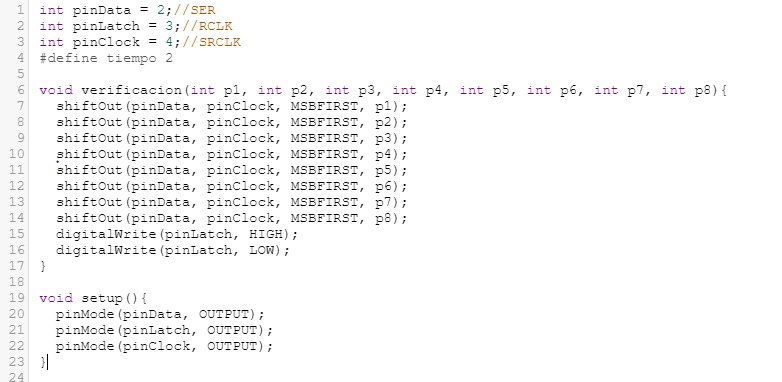
\includegraphics[width=10cm]{Definicion de los puertos.jpeg}
\centering
\caption{Definicion de los puertos}
\label{fig:gestion}
\end{figure}


\begin{figure}[h]
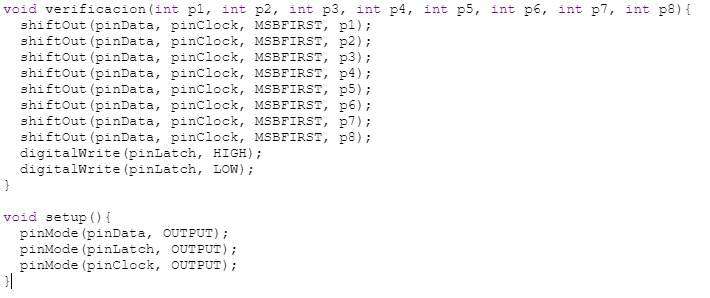
\includegraphics[width=10cm]{Funciones y configuracion de pines.jpeg}
\centering
\caption{Funiones y configuracion de pines}
\label{fig:gestion}
\end{figure}



 \vspace{5cm}




\subsection{Problemas que se presentaron}

Al empezar el montaje del sistema en tinkercar, hubo muchos errores en la conexion de los componentes, obligandonos a recrear en muchas ocasiones la reestructuracion del sistema, debiido que a veces funcionaba pero para la implementacion del codigo manejarlo con una matriz no seria efectivo y traeria futuros problemas.
 \vspace{1cm}
 
  \vspace{1cm}
 
 Al principio ibamos a usar 8 integrados para las filas y 8 integrados para controlar las señales de las coumnas pero luego de analizarlo, nos dimos cuenta que no seria una forma factible para su desarrollo, ya que era mas complicado la manipulacion del pulso y los datos de entrada, a travez del pin de datos "SER"
No entendimos como conectar la matriz al comienzo, por lo que buscabamos los diagramas esquematicos de los leds. 
 \vspace{1cm}


Tuvimos dificultades sobre como encender los leds, y luego buscando como mantenerlos encendidos.
 \vspace{1cm}

Hubo dificultades en el entendimiento del integrado, ya que no contabamos con la experiencia de la electronica y con un programa como arduino.
 \vspace{1cm}

Implementacion del codigo en c++, ya que se hicieron dos versiones, una con un triple arreglo y la otra con memoria dinamica, un triple puntero, haciendo que el codigo al implementarlo en arduino nos diera fallas de manejar los datos de la matriz, en c++ el codigo funcionaba con lo esperado pero en arduino no fue asi.

 \vspace{1cm}

Luego de crear la interfaz, se hicieron las funciones de la matriz para que el usuario fuera rellenandolas con los datos en cada posicion, para imprimir el patron que deseara.
 \vspace{1cm}




 \vspace{1cm}
 Posteriormente pensamos implementar transistores con el objetivo de poder switchear la señal para indicar cual led iba a prender, pero se nos fue indicado que no era permitido.
 
\vspace{1cm}

Los patrones ingresados por el usuario quedan guardados en la matriz pero al momento de hacer el recorrido de las filas/columnas y que envien los pulsos de salida para que se encienda o apague el led estaba fallando.

Los datos que ingresados no se interpretan de la logica estudiada, por ejemplo si se ingresa un dato entero el programa lo toma en numero ascii.




\vspace{14cm}

\subsection{Solucion a problematicas presentadas}

 En la implementacion de las soluciones y empezar a crear el codigo en c++ con arreglo de dos dimensiones, pero el usuario solo podia ingresar un patron, y en caso de que quisiera entrar "Hola" no se podria, por ende se necesito hacer un arreglo de tres dimensiones o un triple puntero, para que pueda guardar cada patron y al final mostrar todos los punteros.
 
   \vspace{1cm}
   
 
 Luego decidimos usar 8 integrados para controlar las 8 filas de la matriz, usando 3 pines digitales del arduino para el control de la señal, para controlar las señales que recibe el integrado.
 Cada integrado usara la salida inversa de la anterior como dato de entrada del integrado siguiente, excepto el ultimo que tiene el pin de salida inversa libre.
 Mas adelante se empezo a realizar la codificacion y configuration de los puertos del arduino como salidas digitales. 
 
 
\begin{figure}[h]
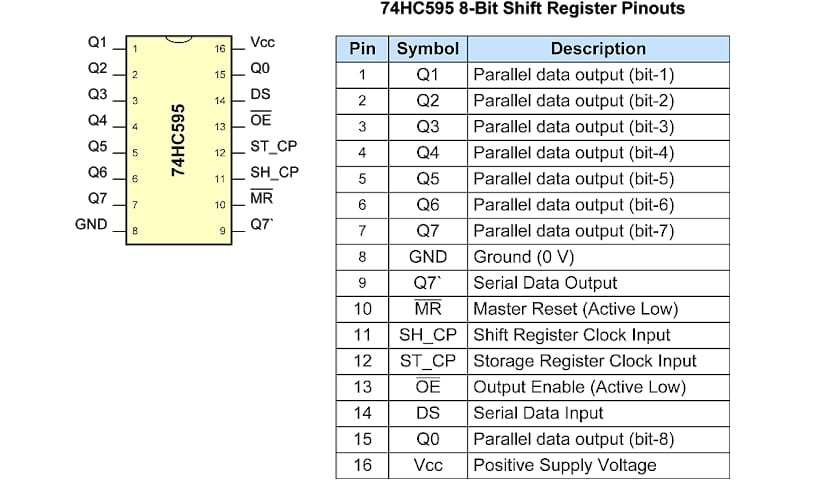
\includegraphics[width=10cm]{Pines integrado2.jpeg}
\centering
\caption{Pines del integrado}
\label{fig:gestion}
\end{figure}

  \vspace{7cm}
  
  Al darnos cuenta que el programa no funcionaba ingresando dato por dato de la matriz, en la funcion "publik" habra un arreglo de 8 elementos los cuales son las filas, y cada elemento sera un numero real, que se convertira en binario, enviando los pulsos de 1 y 0 para encender/apagar led.
  
   \vspace{1cm}
   
   Despues de montar la idea de trabajar con sistema binario, y montar el codigo en c++, pasarlo a arduino nos trajo multiples errores, ya que no se trabaja igual los datos de entrada y las funciones trabajadas no cumplieron llo esperado.
  
  \vspace{1cm}
  
 Entrar numeros binarios y hacer la conversion a entero para que el arreglo lo leyera no fue posible por falta de tiempo, entonces buscamos que el usuario entrara los numeros decimales, que es el equivalente a los 8 bits, para que fuera leyendo fila por fila.
 
   \vspace{1cm}
   
   Como el arreglo era leido de derecha a izquierda y se nos estaba agotando el tiempo para la entrega, se le dio un giro de 180 grados al arduino para que imprimiera el patron en la forma indicada.
 
 
   \vspace{1cm}
 
\begin{figure}[h]
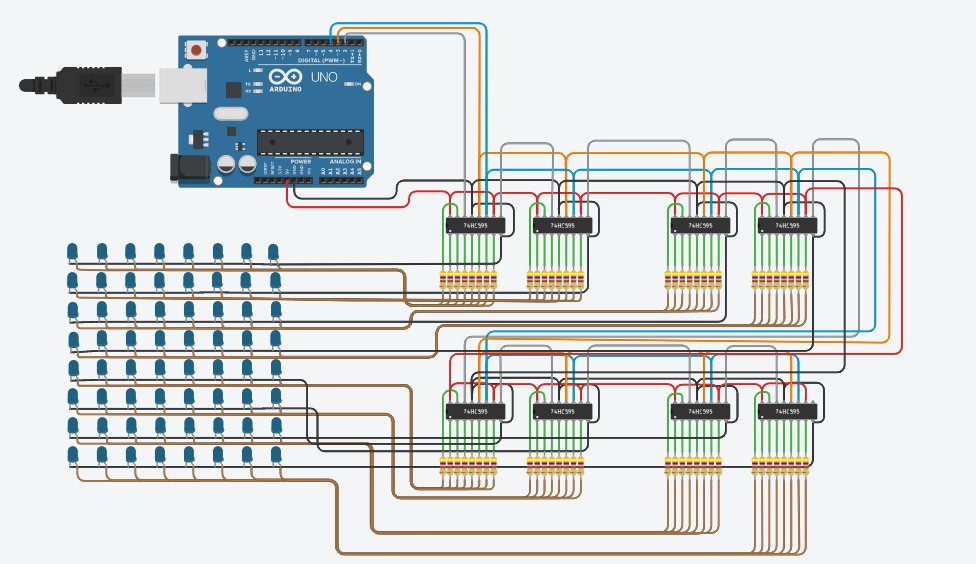
\includegraphics[width=10cm]{Tinkercad.jpeg}
\centering
\caption{Tinkercad}
\label{fig:gestion}
\end{figure}

 \vspace{2cm}
 
\textbf{Codigo de tinkercad listo} 
  
  \begin{verbatim}

CODIGO DEFINITIVO 
int pinData = 2;//SER
int pinLatch = 3;//RCLK
int pinClock = 4;//SRCLK
#define tiempo 400

int **Patrones=NULL;
int n=0;

void publik(int &n,int **patrones){
  for(int i=0;i<n;i++){
    for(int j=0;j<8;j++){
      shiftOut(pinData, pinClock, MSBFIRST, Patrones[i][0]);delay(tiempo);
      shiftOut(pinData, pinClock, MSBFIRST, Patrones[i][1]);delay(tiempo);
      shiftOut(pinData, pinClock, MSBFIRST, Patrones[i][2]);delay(tiempo);
      shiftOut(pinData, pinClock, MSBFIRST, Patrones[i][3]);delay(tiempo);
      shiftOut(pinData, pinClock, MSBFIRST, Patrones[i][4]);delay(tiempo);
      shiftOut(pinData, pinClock, MSBFIRST, Patrones[i][5]);delay(tiempo);
      shiftOut(pinData, pinClock, MSBFIRST, Patrones[i][6]);delay(tiempo);
      shiftOut(pinData, pinClock, MSBFIRST, Patrones[i][7]);delay(tiempo);
      digitalWrite(pinLatch, HIGH);
      digitalWrite(pinLatch, LOW);
    }
    shiftOut(pinData,pinClock,MSBFIRST, 0);
      shiftOut(pinData,pinClock,MSBFIRST, 0);
      shiftOut(pinData,pinClock,MSBFIRST, 0);
      shiftOut(pinData,pinClock,MSBFIRST, 0);
      shiftOut(pinData,pinClock,MSBFIRST, 0);
      shiftOut(pinData,pinClock,MSBFIRST, 0);
      shiftOut(pinData,pinClock,MSBFIRST, 0);
      shiftOut(pinData,pinClock,MSBFIRST, 0);
  }
}
  
void imagen(int &n){
  Serial.println("Bienvenido a la funcion Imagen ingrese el valor de la primer posicion: ");
  //while(Serial.available()<=0){
  //}
  Patrones=new int*[n];
  for(int i=0;i<n;i++){
   	Patrones[i]=new int[8];
    for(int j=0;j<8;j++){
      while(Serial.available()<=0){
      }
      Serial.print("Ingrese el valor de: ");
      Serial.print("[");
      Serial.print(i);
      Serial.print("]");
      Serial.print("[");
      Serial.print(j);
      Serial.print("]");
      Serial.print(": ");
      Serial.println();
      Patrones[i][j]=Serial.parseInt();
      Serial.println(Patrones[i][j]);
    }
    
  }
}


int verificacion(int p1,int p2,int p3,int p4,int p5, int p6, int p7, int p8){
  	shiftOut(pinData, pinClock, MSBFIRST, p1);
  	shiftOut(pinData, pinClock, MSBFIRST, p2);
  	shiftOut(pinData, pinClock, MSBFIRST, p3);
  	shiftOut(pinData, pinClock, MSBFIRST, p4);
  	shiftOut(pinData, pinClock, MSBFIRST, p5);
  	shiftOut(pinData, pinClock, MSBFIRST, p6);
  	shiftOut(pinData, pinClock, MSBFIRST, p7);
  	shiftOut(pinData, pinClock, MSBFIRST, p8);
  	digitalWrite(pinLatch, HIGH);
  	digitalWrite(pinLatch, LOW);
}

void setup()
{
  pinMode(pinData,OUTPUT);
  pinMode(pinLatch,OUTPUT);
  pinMode(pinClock,OUTPUT);
  Serial.begin(9600);
}

void loop(){
  	Serial.println("MENU DE FUNCIONAMIENTO");
    Serial.println("1. FUNCION DE VERIFICACION");
    Serial.println("2. FUNCION IMAGEN");
    Serial.println("3. FUNCION PUBLIK");
    while(Serial.available()==0){
    }
      int opcion=Serial.parseInt();
      switch(opcion){
      	case 1:
        Serial.println("EJECUTANDO VERIFICACION");
        //for(int j=0;j<9;j++){
            //int pot=pow(2,j);
        	verificacion(0,0,0,0,0,0,0,255);delay(tiempo);
            verificacion(0,0,0,0,0,0,255,0);delay(tiempo);
            verificacion(0,0,0,0,0,255,0,0);delay(tiempo);
            verificacion(0,0,0,0,255,0,0,0);delay(tiempo);
            verificacion(0,0,0,255,0,0,0,0);delay(tiempo);
            verificacion(0,0,255,0,0,0,0,0);delay(tiempo);
            verificacion(0,255,0,0,0,0,0,0);delay(tiempo);
            verificacion(255,0,0,0,0,0,0,0);delay(tiempo);
        //}
        verificacion(0,0,0,0,0,0,0,0);
        break;
        case 2:
        Serial.println("cantidad de patrones que desea ingresar: ");
  		while(Serial.available()<=0){
  		}
  		n=Serial.parseInt();
  		Serial.println(n);
  		imagen(n);
        break;
        case 3:
        publik(n,Patrones);
        verificacion(0,0,0,0,0,0,0,0);
        break;
      }
    
}

\end{verbatim}

\vspace{7cm}

\section{Conclusion} \label{conclulsion}

Se soluciono el problema planteado con todas las problematicas estipuladas y siguiendo los parametros señalados. Se necesito de mucha investigacion para la estructura del arduino, en el uso de sus componentes, conociendo su manejo e infraestructura, al igual que la sintaxis que maneja arduino, que es diferente a c++, que fue donde planteamos la idea de desarrollo.

\vspace{1cm}

Se fallo en multiples ocasiones en la infraestructura del arduino y en la implementacion del codigo, pero fue necesario para comprender su funcionamiento.

\vspace{13cm}

\section{Manual de uso} \label{Manual de uso}

El programa sirve para usted pueda ingresar patrones y por medio de 64 leds va a mostrar dichos patrones.

\vspace{1cm}

\textbf{MENU} \\
\\
En el menu habran 4 opciones y el usuaria debe ingresar el numero de la opcion a ejecutar :\\
1. Verificar: Comprueba que todos los leds encienden. \\
2. Imagen: Agregar el patron que desea mostrar en los leds.\\
3. Publik: Mostrar el patron ingresado en "Imagen" ( en caso que no halla ingresado el patron no se encendera ningun led ).\\
4.Reiniciar: Eliminar los patrones ingresados en la opcion 2.

\vspace{1cm}

\textbf{EL USUARIO DESEA INGRESAR PATRON(ES) Y OBSERVARLOS EN LOS LEDS} 

\vspace{1cm}

Opcional: Darle en la opcion 1, para verificar que todos los leds enciendan.\\

1. Darle en el menu la opcion 2, para empezar a ingresar el/los patrones.\\
2. El programa le va a pedir la cantidad de patrones a ingresar.\\
3. El programa le va a empezar a pedir un numero entero entre 0 y 255, 8 veces, que son las 8 filas de los leds.\\
4. Tomando como base que 1 es encendido y 0 es apagado, ingrese el numero entero que signifique en codigo binario los leds que desea tener encendidos o apagados, teniendo en cuenta que se lee de derecha a izquierda. \\
Ejemplo: si en la primera fila desea encender las columnas 3,5,7 eso significario en binario: 01010100 , pero el usuario deberia ingresar su equivalencia en entero que en este caso seria: 84.\\

5. En caso de que haya pedido mas de 1 patron a dibujar, apenas termine de ingresar los 8 elementos, el programa le seguira pidiendo los otros 8 elementos, hasta que termine el numero de patrones que se ingreso en un principio.\\

6. El programa le retornara al menu, e ingrese la opcion 3 ( Publik ) donde le empezara a encender los leds correspondientes a los patrones ingresados.\\



\end{document}
